\documentclass{article}
\usepackage[utf8]{inputenc}
\usepackage{tikz}
\usetikzlibrary{automata, positioning, arrows}
\usepackage{amsmath}
\usepackage{algorithm}
\usepackage[noend]{algpseudocode}
\title{Code and Architecture Example}
\author{}
\date{}
\begin{document}
\maketitle
\tikzset{
         ->,  % makes the edges directed
         >=stealth, % makes the arrow heads bold
         node distance=3cm, % specifies the minimum distance between two nodes. Change if necessary.
         every state/.style={thick, fill=gray!10}, % sets the properties for each ’state’ node
         initial text=$ $, % sets the text that appears on the start arrow
         }

\section{Intro}
Ros is an open-source robotics middleware suite. Although ROS is not an operating system (OS) but a set of software frameworks for robot software development, it provides services designed for a heterogeneous computer cluster such as hardware abstraction, low-level device control, implementation of commonly used functionality, message-passing between processes, and package management. (stole definition from Wikipedia)

\section{Publisher Subscriber Architecture Model}
\begin{figure}[htp]
    \centering
    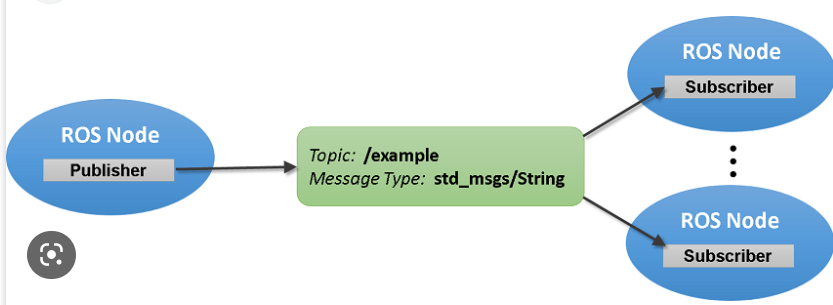
\includegraphics[width=12cm]{pubsub.png}
    \caption{}
    \label{fig:pubsub}
\end{figure}


\textbf{Nodes:} Are usually associated with a python script or c++ object. Nodes can do two main things - publish and subscribe. A node can be both a publisher and a subscriber.\\\\
\textbf{Publisher node: } Publish(send) data to a topic(Represented by outing edges in figure above). \\\\
\textbf{Subscriber node: } Subscribes(listens) to data from a topic(Represented by incoming edges in figure above), then uses a callback function to create desired output from topic data. \\\\
\textbf{Topics: } Are the name handlers for where nodes will publish and subscribe to data.\\\\
\textbf{Ros messages: } Are objects predefined in ros or defined by the programmer that can be transmitted over topics. 
\section{System Design}
Ros programming is often done using a top to bottom approach. The engineer must design the system architecture(as shown above), then develop(code) the individual nodes of the system.\\\\
\textbf{Advantages:} \\
1. Simplifies documentation and readability of the system.\\
2. Stores code in modular nodes that can be easily added and removed to any system(increases code re-usability).\\
3. Increased programming efficiency since nodes can be written in different languages and are allowed to communicate within a ros environment.\\
4. Ros nodes communicate using asynchronous message passing, which improves performance by simplifying parallelism and making it more accessible to developers.

\section{Whats a callback function?}
Publisher nodes send data to topics, and subscriber nodes collect data from topics. Each time a subscriber node receives data from a topic, the subscriber node will run a callback function. A callback function is a function, that receives data(input) from a topic asynchronously, and computes the output in separate thread. Each time data is received from a topic a new thread opens and runs the callback function. 

\section{Whats a point cloud?}
A point cloud is a set of 3d points within some frame. Example of devices that gather point cloud data are kinect(xbox), lidar(similar to radar), and stereo camera(uses two rgb cameras to triangulate 3d points). 
\section{Example of architecture}
Design a system  architecture using the publisher-subscriber model that from 2D object inferences, the robot moves it head in 
the direction of individual people. If there is more than one person, the robot creates a list of 
centroids(representing the people) and iterates through this list by pointing its head at each person for three seconds. 
The robot has two measuring devices, a camera which outputs rgb images of what the robot is looking at, 
and a kinect device that outputs a point-cloud of 3D points measured in the same frame as the camera.\\\\\\
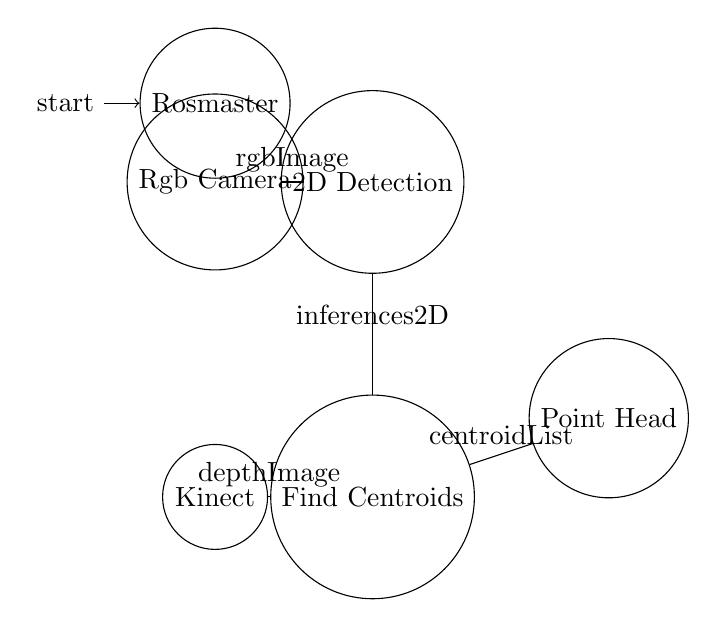
\begin{tikzpicture}
    % tikz code goes here
    \node[state, initial] (1) {Rosmaster};
    \node[state, below of=1] (2) {Rgb Camera};
    \node[state, below of=2] at (0, -4) (3) {Kinect};
    \node[state, below of=1, right of=2] at (1,0) (4) {2D Detection};
    \node[state, below of=2, right of=3] at (1,-4) (5) {Find Centroids};
    \node[state, right of=5] at (4,-4) (6) {Point Head};

    \draw   (2) edge[above] node{rgbImage} (4)
            (3) edge[above] node{depthImage} (5)
            (4) edge[above] node{inferences2D} (5)
            (5) edge[above] node{centroidList} (6);
\end{tikzpicture}
\label{fig:my_label}

\section{Relating your first run to the publisher subscriber model}
Remember to run in each terminal you open:\\
1. cd catkin\_ws\\ 
2. source devel/setup.bash\\
\textbf{Roscore}- Running roscore in a separate terminal will set up your ros master node for the system. The ros master node, is a node that manages all other nodes and topics created by the user. \\\\
\textbf{rosrun}- This command runs and adds a node to your architecture.\\\\
examples(run each in a new terminal):\\ 
rosrun talk\_listen listener.py\\ 
rosrun talk\_listen talker.py\\\\
The argument test\_run is a package, for now think of a package as a  set of nodes that defines an architecture.\\\\
listener.py is the python script that runs the node listener, which subscribes to topic chatter.\\\\
talker.py is the python script that runs the node talker, which publishes to the topic chatter. \\
(code provided on blackboard please review!)\\\\
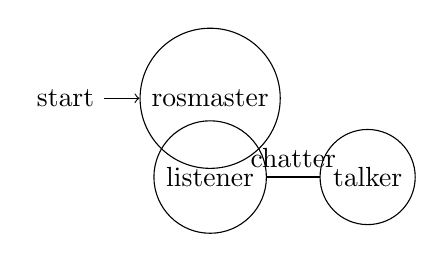
\begin{tikzpicture}
    % tikz code goes here
    \node[state, initial] (1) {rosmaster};
    \node[state, below of=1] (2) {listener};
    \node[state, below of=1, right of=2] at (1,0) (3) {talker};

    \draw   (2) edge[above] node{chatter} (3);
\end{tikzpicture}\\\\
To view this architecture in ros(for debugging and making sure everything is correct) run the command: \\
\textbf{rosrun rqt\_graph rqt\_graph}

\section{Turtlesim}
First lets start by running roslaunch command. The roslaunch command allows you to launch multiple nodes and the rosmaster with just one command.\\
example: \emph{roslaunch turtle\_motion turtle\_clean.launch} \\(remember to create the package as instructed in the ROS\_Instructions pdf available on blackboard.)\\\\
If nothing happens on the turtle simulator, open up the file catkin\_ws/src/turtle\_motion/src/grid\_clean.py and call any of the functions included from there in the main function.\\\\
This command will run your rosmaster, rosrun turtlesim turtlesim\_node, and rosrun turtle\_motion grid\_clean.py all in one terminal and you do not have to worry about managing multiple nodes across multiple terminals.\\\\
\begin{figure}[htp]
    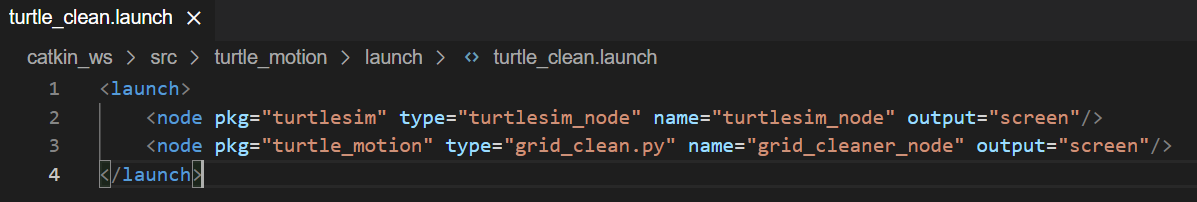
\includegraphics[width=12cm]{launchfile.png}
    \label{fig:launch}
\end{figure} 
The important things to note about this file is that you must start and end the file with the launch tag ($<$launch$>$).  Each node you set up begins with a node tag($<$node$>$) and then you must specify the package where the node is contained(pkg=), the name of the file that sets up the node(type=), and the name of the node(name=); all other arguments are optional.
\newpage

\begin{figure}[htp]
    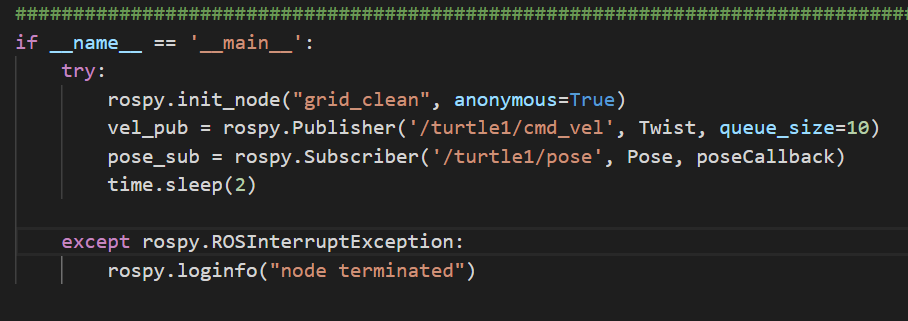
\includegraphics[width=12cm]{main.png}
    \label{fig:mainy}
\end{figure} 
The image above shows how we set up the node, publisher and subscriber. Note that every time you set up a publisher or subscriber you must both provide a topic name and a message type.Example: rospy.Subscriber(topic\_name, msg\_type, callback function name). The callback function is written by the programmer, and it is the code that is executed every time the node receives a message on a topic.\\\\

\begin{figure}[htp]
    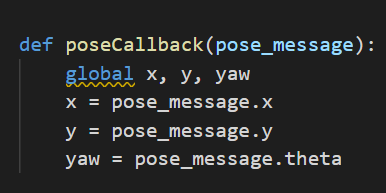
\includegraphics[width=10cm]{callback.png}
    \label{fig:callback}
\end{figure} 
Example of callback in code that updates variables x, y, and yaw based on the robots current position on the simulator.\\\\
\newpage 

\begin{figure}[htp]
    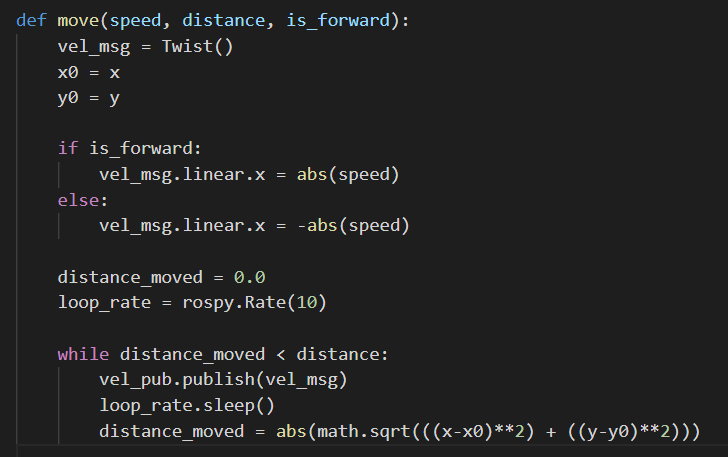
\includegraphics[width=10cm]{move.png}
    \label{fig:move}
\end{figure} 
The move function has the robot move at some speed linear.x by publishing to the /turtle1/cmd\_vel topic. The message type of this topic is geometry\_msgs/Twist. This message has two member variables Vector3 linear and Vector3 angular. The linear variable sets the linear velocity of the turtle and the angular variable sets the angular velocity of the turtle robot. In the code we use the distance formula to compute how much the robot has moved from its initial position.\\\\

\begin{figure}[htp]
    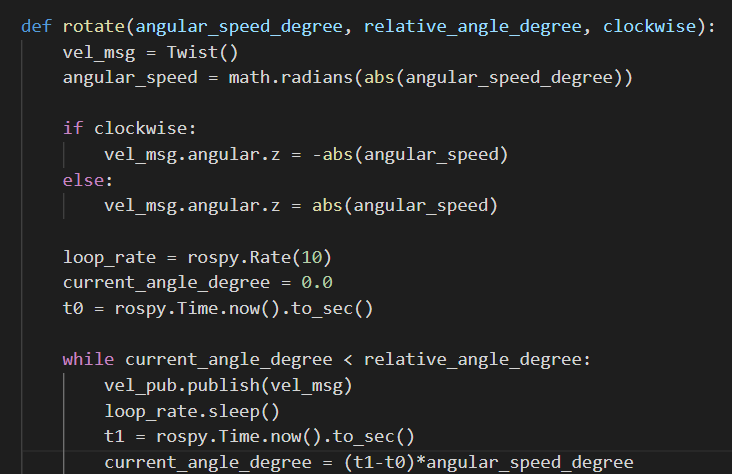
\includegraphics[width=10cm]{rotate.png}
    \label{fig:rotate}
\end{figure} 
The rotate function also publishes /turtle1/cmd\_vel topic and uses a message type of geometry\_msgs/Twist. This time we are interested 
in the member variable Vector3 angular which sets the rotational velocity of the robot. The speed input parameter tells us how fast our turtle robot will rotate per second, and the idea is to rotate for however many seconds are required to reach our goal. 
\subsection{turtle architecture}
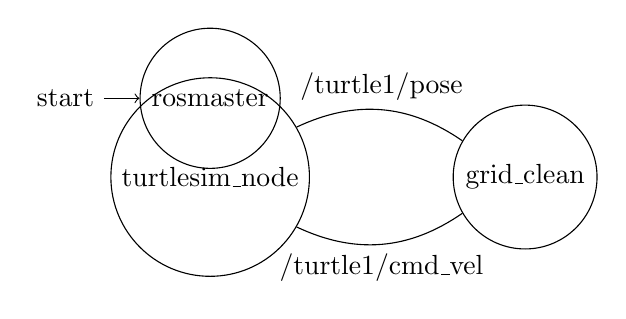
\begin{tikzpicture}
    % tikz code goes here
    \node[state, initial] (1) {rosmaster};
    \node[state, below of=1] (2) {turtlesim\_node};
    \node[state, below of=1, right of=2] at (3,0) (3) {grid\_clean};

    \draw   (2) edge[above] [bend left] node{/turtle1/pose} (3) 
            (3) edge[below] [bend left] node{/turtle1/cmd\_vel} (2);
\end{tikzpicture}

\newpage

\section{Website Server Ros Setup}
\textbf{1.} Create an account on theconstructsim.com\\\\
\textbf{2.} In the left hand column, click on my "rosjects" then click on create "new rosject".\\\\
\textbf{3.} Name your rosject whatever you would like but make sure to select ros distro as "Ros melodic".\\\\
\textbf{4.} There will be a tool bar at the bottom of the screen when you open your project. From this tool bar you will be using the following: Web shell, Code editor, grapical tools.

\section{Environment Setup}
\textbf{1.} Create a folder name catkin\_ws. Create a sub-folder inside of catkin\_ws named src. catkin\_ws will be your local working environment for ros.\\\\
\textbf{2.} Run the command \emph{cd $\sim$/catkin\_ws} followed by \emph{catkin\_make}. The command catkin\_make converts a regular folder into a ros repository.\\\\
\textbf{3.} Every time you open a web shell or new tabs in web shell run \emph{source $\sim$/catkin\_ws/devel/setup.bash}. This command sets your working environment in the current shell to the repo catkin\_ws. Otherwise you will be running from its installation working environment. 

\section{Creating ros packages}
\textbf{1.} A ros package is a small standalone ros project created inside of your ros repository.\\\\
\textbf{2.}  Run \emph{cd $\sim$/catkin\_ws/src} followed by, \emph{catkin\_create\_pkg [name of package] [depend1] [depend2] ...}\\
An example(Do it!): \emph{catkin\_create\_pkg talk\_listen std\_msgs roscpp rospy}\\\\
\textbf{3.} After creating a package make sure to execute steps 2 and 3 from section Environment Setup.

\section{First Example}
\textbf{1.} On blackboard under course materials you will find a folder called ros\_examples, and inside this folder another folder called talk\_listen\_stuff. Copy the files "listener.py" and "talker.py" into $\sim$/catkin\_ws/src/talk\_listen/src.\\\\
\textbf{2.} Make sure files are executable by running \emph{chmod +x  $\sim$/catkin\_ws/src/talk\_listen/src/listener.py} and \emph{chmod +x  $\sim$/catkin\_ws/src/talk\_listen/src/talker.py}\\\\
\textbf{3.} In your current shell run the command \emph{roscore}, this will set up a ros master node that will manage all future nodes.\\\\
\textbf{4.} open a new tab in your web shell, run \emph{source $\sim$/catkin\_ws/devel/setup.bash} followed by \emph{rosrun talk\_listen listener.py}\\\\
\textbf{5.} open a third tab in your web shell, run \emph{source $\sim$/catkin\_ws/devel/setup.bash} followed by \emph{rosrun talk\_listen talker.py}\\\\
\textbf{6.} The steps in this section should result in basic stdout output in the terminal where you ran the listener node (\emph{rosrun talk\_listen listener.py}). Congrats you just ran your first ros system!

\section{More}
Moving forward you will just need to create two more packages for the homework(run these in $\sim$/catkin\_ws/src):\\\\
1. \emph{catkin\_create\_pkg turtle\_motion std\_msgs roscpp rospy}\\\\
2. \emph{catkin\_create\_pkg learn\_tf2 tf2 tf2\_ros roscpp rospy turtlesim}\\\\
Use the examples in ros\_examples(on blackboard) to test these projects out.

\end{document}
